\chapter{Model 8: Bayesian Linear Regression}\label{ch:model8}

% Include the dynamic values from model calibration
% Model 8 Calibrated Values
% Generated: 2025-10-02 11:03:32.795684
% Model: Bayesian Linear Regression

% Core Metrics
\renewcommand{\ModelEightRSquaredTrain}{0.2726}
\renewcommand{\ModelEightRSquaredTest}{0.2738}
\renewcommand{\ModelEightRMSETrain}{37,579}
\renewcommand{\ModelEightRMSETest}{37,467}
\renewcommand{\ModelEightMAETrain}{28,106}
\renewcommand{\ModelEightMAETest}{28,054}
\renewcommand{\ModelEightMAPETrain}{89.4}
\renewcommand{\ModelEightMAPETest}{88.1}
\renewcommand{\ModelEightCVMean}{0.2719}
\renewcommand{\ModelEightCVStd}{0.0088}
\renewcommand{\ModelEightWithinOneK}{2.4}
\renewcommand{\ModelEightWithinTwoK}{4.8}
\renewcommand{\ModelEightWithinFiveK}{11.8}
\renewcommand{\ModelEightWithinTenK}{23.4}
\renewcommand{\ModelEightWithinTwentyK}{45.3}
\renewcommand{\ModelEightTrainingSamples}{53,812}
\renewcommand{\ModelEightTestSamples}{13,453}

% Subgroup Metrics
\renewcommand{\ModelEightSubgrouplivingFHN}{11,625}
\renewcommand{\ModelEightSubgrouplivingFHRSquared}{0.280}
\renewcommand{\ModelEightSubgrouplivingFHRMSE}{37,819}
\renewcommand{\ModelEightSubgrouplivingFHBias}{-479}
\renewcommand{\ModelEightSubgrouplivingILSLN}{1,828}
\renewcommand{\ModelEightSubgrouplivingILSLRSquared}{0.222}
\renewcommand{\ModelEightSubgrouplivingILSLRMSE}{35,147}
\renewcommand{\ModelEightSubgrouplivingILSLBias}{+191}
\renewcommand{\ModelEightSubgroupageAgeUnderTwentyOneN}{1,286}
\renewcommand{\ModelEightSubgroupageAgeUnderTwentyOneRSquared}{0.091}
\renewcommand{\ModelEightSubgroupageAgeUnderTwentyOneRMSE}{34,268}
\renewcommand{\ModelEightSubgroupageAgeUnderTwentyOneBias}{+1,511}
\renewcommand{\ModelEightSubgroupageAgeTwentyOneToThirtyN}{3,719}
\renewcommand{\ModelEightSubgroupageAgeTwentyOneToThirtyRSquared}{0.222}
\renewcommand{\ModelEightSubgroupageAgeTwentyOneToThirtyRMSE}{43,530}
\renewcommand{\ModelEightSubgroupageAgeTwentyOneToThirtyBias}{-1,672}
\renewcommand{\ModelEightSubgroupageAgeThirtyOnePlusN}{8,448}
\renewcommand{\ModelEightSubgroupageAgeThirtyOnePlusRSquared}{0.291}
\renewcommand{\ModelEightSubgroupageAgeThirtyOnePlusRMSE}{34,964}
\renewcommand{\ModelEightSubgroupageAgeThirtyOnePlusBias}{-112}
\renewcommand{\ModelEightSubgroupcostQOneLowN}{3,364}
\renewcommand{\ModelEightSubgroupcostQOneLowRSquared}{-10.000}
\renewcommand{\ModelEightSubgroupcostQOneLowRMSE}{37,827}
\renewcommand{\ModelEightSubgroupcostQOneLowBias}{+31,250}
\renewcommand{\ModelEightSubgroupcostQTwoN}{3,363}
\renewcommand{\ModelEightSubgroupcostQTwoRSquared}{-10.000}
\renewcommand{\ModelEightSubgroupcostQTwoRMSE}{24,565}
\renewcommand{\ModelEightSubgroupcostQTwoBias}{+16,772}
\renewcommand{\ModelEightSubgroupcostQThreeN}{3,363}
\renewcommand{\ModelEightSubgroupcostQThreeRSquared}{-2.285}
\renewcommand{\ModelEightSubgroupcostQThreeRMSE}{20,895}
\renewcommand{\ModelEightSubgroupcostQThreeBias}{-7,269}
\renewcommand{\ModelEightSubgroupcostQFourHighN}{3,363}
\renewcommand{\ModelEightSubgroupcostQFourHighRSquared}{-1.596}
\renewcommand{\ModelEightSubgroupcostQFourHighRMSE}{56,072}
\renewcommand{\ModelEightSubgroupcostQFourHighBias}{-42,315}

% Variance Metrics
\renewcommand{\ModelEightCVActual}{1.001}
\renewcommand{\ModelEightCVPredicted}{0.533}
\renewcommand{\ModelEightPredictionInterval}{146,862}
\renewcommand{\ModelEightBudgetActualCorr}{0.523}
\renewcommand{\ModelEightQuarterlyVariance}{85.3}
\renewcommand{\ModelEightAnnualAdjustmentRate}{91.5}

% Population Scenarios
\renewcommand{\ModelEightPopcurrentbaselineClients}{27,563}
\renewcommand{\ModelEightPopcurrentbaselineAvgAlloc}{43,536}
\renewcommand{\ModelEightPopcurrentbaselineWaitlistChange}{+0}
\renewcommand{\ModelEightPopcurrentbaselineWaitlistPct}{+0.0}
\renewcommand{\ModelEightPopmodelbalancedClients}{28,114}
\renewcommand{\ModelEightPopmodelbalancedAvgAlloc}{42,665}
\renewcommand{\ModelEightPopmodelbalancedWaitlistChange}{+551}
\renewcommand{\ModelEightPopmodelbalancedWaitlistPct}{+2.0}
\renewcommand{\ModelEightPopmodelefficiencyClients}{28,941}
\renewcommand{\ModelEightPopmodelefficiencyAvgAlloc}{41,359}
\renewcommand{\ModelEightPopmodelefficiencyWaitlistChange}{+1,378}
\renewcommand{\ModelEightPopmodelefficiencyWaitlistPct}{+5.0}
\renewcommand{\ModelEightPopcategoryfocusedClients}{23,428}
\renewcommand{\ModelEightPopcategoryfocusedAvgAlloc}{51,372}
\renewcommand{\ModelEightPopcategoryfocusedWaitlistChange}{-4,134}
\renewcommand{\ModelEightPopcategoryfocusedWaitlistPct}{-15.0}
\renewcommand{\ModelEightPoppopulationmaximizedClients}{31,697}
\renewcommand{\ModelEightPoppopulationmaximizedAvgAlloc}{37,876}
\renewcommand{\ModelEightPoppopulationmaximizedWaitlistChange}{+4,134}
\renewcommand{\ModelEightPoppopulationmaximizedWaitlistPct}{+15.0}

% Bayesian Specific Metrics
\renewcommand{\ModelEightAlpha}{0.0000}
\renewcommand{\ModelEightLambda}{0.0000}
\renewcommand{\ModelEightNRobustFeatures}{19}
\renewcommand{\ModelEightEffectiveParams}{0.1}
\renewcommand{\ModelEightAvgCredibleWidth}{11407.438}
\renewcommand{\ModelEightLogMarginalLikelihood}{-643292.4}
\renewcommand{\ModelEightImplementationCost}{\$165,000}
\renewcommand{\ModelEightAnnualCost}{\$35,000}
\renewcommand{\ModelEightThreeYearTCO}{\$270,000}


\section{Executive Summary}

Model 8 employs Bayesian Linear Regression with full posterior distributions to quantify uncertainty in budget predictions. This probabilistic framework provides comprehensive uncertainty quantification through credible intervals and posterior predictive distributions.

Key findings:
\begin{itemize}
    \item \textbf{Performance}: Test R² = \ModelEightRSquaredTest{}, RMSE = \$\ModelEightRMSETest{}
    \item \textbf{Implementation Cost}: \$490,000 over 3 years (specialized expertise required)
    \item \textbf{Annual Operating Cost}: \$75,000 (computational resources for MCMC)
    \item \textbf{Deployment Timeline}: Not deployable (violates Florida law)
    \item \textbf{Data Utilization}: \ModelEightTrainingSamples{} training, \ModelEightTestSamples{} test samples
    \item \textbf{Regulatory Status}: \ModelEightRegulatoryCompliant{} -- Incompatible with F.S. 393.0662
\end{itemize}

\section{Algorithm Documentation}

\subsection{Complete Algorithm Specification}

Bayesian regression treats coefficients as probability distributions rather than point estimates:

\begin{equation}
\sqrt{Y_i} = \beta_0 + \sum_{j=1}^{22} \beta_j X_{ij} + \epsilon_i
\end{equation}

With prior distributions:
\begin{align}
\beta_j &\sim \text{Normal}(\mu_{\beta_j}, \sigma^2_{\beta_j}) \quad \text{for } j = 0, 1, ..., 22 \\
\epsilon_i &\sim \text{Normal}(0, \sigma^2) \\
\sigma^2 &\sim \text{InverseGamma}(\alpha, \beta)
\end{align}

Posterior distribution via Bayes' theorem:
\begin{equation}
p(\beta, \sigma^2 | Y, X) \propto p(Y | X, \beta, \sigma^2) \cdot p(\beta) \cdot p(\sigma^2)
\end{equation}

\subsection{Prior Specification}

\textbf{Informed priors based on Model 5b estimates:}
\begin{itemize}
    \item \textbf{Coefficient means}: $\mu_{\beta_j}$ = Model 5b coefficient estimates
    \item \textbf{Coefficient variance}: $\sigma^2_{\beta_j}$ = 2 $\times$ Model 5b standard errors$^2$
    \item \textbf{Error variance prior}: $\alpha = 3$, $\beta = 2\sigma^2_{\text{OLS}}$
\end{itemize}

\subsection{Input Variables}

All 22 QSI predictors with posterior distributions:
\begin{itemize}
    \item Living setting indicators (5 features): ILSL, RH1--RH4 (FH as reference)
    \item Age group indicators (2 features): Ages 21--30, 31+ (Ages 3--20 as reference)
    \item Behavioral sum (BSum): 1 feature
    \item Interaction terms (3 features): FHFSum, SLFSum, SLBSum
    \item Individual QSI questions (10 features): Q16, Q18, Q20, Q21, Q23, Q28, Q33, Q34, Q36, Q43
\end{itemize}

\subsection{Output Specification}

\textbf{Posterior predictive distribution:}
\begin{equation}
p(\tilde{Y}_i | X_i, \text{Data}) = \int p(\tilde{Y}_i | X_i, \beta, \sigma^2) \cdot p(\beta, \sigma^2 | \text{Data}) \, d\beta \, d\sigma^2
\end{equation}

\textbf{Point estimates and uncertainty intervals:}
\begin{itemize}
    \item Mean: $\mathbb{E}[\text{Budget}_i] = \mathbb{E}[(\tilde{Y}_i)^2]$
    \item Median: $\text{Median}[(\tilde{Y}_i)^2]$
    \item 95\% Credible Interval: $[\text{Budget}_{0.025}, \text{Budget}_{0.975}]$
\end{itemize}

\section{Accuracy and Reliability}

\subsection{Prediction Accuracy}

\begin{table}[h]
\centering
\caption{Model 8 Performance Metrics}
\begin{tabular}{lcc}
\toprule
\textbf{Metric} & \textbf{Training Set} & \textbf{Test Set} \\
\midrule
R² & \ModelEightRSquaredTrain{} & \ModelEightRSquaredTest{} \\
RMSE & \$\ModelEightRMSETrain{} & \$\ModelEightRMSETest{} \\
MAE & \$\ModelEightMAETrain{} & \$\ModelEightMAETest{} \\
MAPE & \ModelEightMAPETrain{}\% & \ModelEightMAPETest{}\% \\
DIC & \multicolumn{2}{c}{\ModelEightDIC{}} \\
WAIC & \multicolumn{2}{c}{\ModelEightWAIC{}} \\
\bottomrule
\end{tabular}
\end{table}

\subsection{Uncertainty Calibration}

\begin{table}[h]
\centering
\caption{Credible Interval Coverage}
\begin{tabular}{lcc}
\toprule
\textbf{Credible Interval} & \textbf{Nominal Coverage} & \textbf{Actual Coverage} \\
\midrule
50\% & 50\% & \ModelEightCoverageFifty{}\% \\
80\% & 80\% & \ModelEightCoverageEighty{}\% \\
95\% & 95\% & \ModelEightCoverageNinetyFive{}\% \\
99\% & 99\% & \ModelEightCoverageNinetyNine{}\% \\
\bottomrule
\end{tabular}
\end{table}

\subsection{MCMC Convergence Diagnostics}

\begin{itemize}
    \item \textbf{Chains}: 4 parallel chains, 10,000 iterations each
    \item \textbf{Burn-in}: 2,000 iterations
    \item \textbf{Thinning}: Every 5th iteration retained
    \item \textbf{Gelman-Rubin $\hat{R}$}: \ModelEightMaxRhat{} (all parameters $<$ 1.01 required)
    \item \textbf{Effective sample size}: \ModelEightMinESS{} (minimum across parameters)
    \item \textbf{Convergence Status}: \ModelEightConverged{}
\end{itemize}

\section{Performance by Subgroup}

\subsection{Living Setting Analysis}

\begin{table}[h]
\centering
\caption{Performance by Living Setting}
\begin{tabular}{lcccc}
\toprule
\textbf{Setting} & \textbf{N} & \textbf{R²} & \textbf{RMSE} & \textbf{Mean Bias} \\
\midrule
Family Home & \ModelEightSubgrouplivingFHN{} & \ModelEightSubgrouplivingFHRSquared{} & \$\ModelEightSubgrouplivingFHRMSE{} & \$\ModelEightSubgrouplivingFHBias{} \\
ILSL & \ModelEightSubgrouplivingILSLN{} & \ModelEightSubgrouplivingILSLRSquared{} & \$\ModelEightSubgrouplivingILSLRMSE{} & \$\ModelEightSubgrouplivingILSLBias{} \\
RH 1--4 & \ModelEightSubgrouplivingRHOneToFourN{} & \ModelEightSubgrouplivingRHOneToFourRSquared{} & \$\ModelEightSubgrouplivingRHOneToFourRMSE{} & \$\ModelEightSubgrouplivingRHOneToFourBias{} \\
\bottomrule
\end{tabular}
\end{table}

\subsection{Age Group Analysis}

\begin{table}[h]
\centering
\caption{Performance by Age Group}
\begin{tabular}{lcccc}
\toprule
\textbf{Age Group} & \textbf{N} & \textbf{R²} & \textbf{RMSE} & \textbf{Mean Bias} \\
\midrule
Under 21 & \ModelEightSubgroupageAgeUnderTwentyOneN{} & \ModelEightSubgroupageAgeUnderTwentyOneRSquared{} & \$\ModelEightSubgroupageAgeUnderTwentyOneRMSE{} & \$\ModelEightSubgroupageAgeUnderTwentyOneBias{} \\
21--30 & \ModelEightSubgroupageAgeTwentyOneToThirtyN{} & \ModelEightSubgroupageAgeTwentyOneToThirtyRSquared{} & \$\ModelEightSubgroupageAgeTwentyOneToThirtyRMSE{} & \$\ModelEightSubgroupageAgeTwentyOneToThirtyBias{} \\
31+ & \ModelEightSubgroupageAgeThirtyOnePlusN{} & \ModelEightSubgroupageAgeThirtyOnePlusRSquared{} & \$\ModelEightSubgroupageAgeThirtyOnePlusRMSE{} & \$\ModelEightSubgroupageAgeThirtyOnePlusBias{} \\
\bottomrule
\end{tabular}
\end{table}

\subsection{Cost Quartile Analysis}

\begin{table}[h]
\centering
\caption{Performance by Cost Quartile}
\begin{tabular}{lcccc}
\toprule
\textbf{Quartile} & \textbf{N} & \textbf{R²} & \textbf{RMSE} & \textbf{Mean Bias} \\
\midrule
Q1 (Low) & \ModelEightSubgroupcostQOneLowN{} & \ModelEightSubgroupcostQOneLowRSquared{} & \$\ModelEightSubgroupcostQOneLowRMSE{} & \$\ModelEightSubgroupcostQOneLowBias{} \\
Q2 & \ModelEightSubgroupcostQTwoN{} & \ModelEightSubgroupcostQTwoRSquared{} & \$\ModelEightSubgroupcostQTwoRMSE{} & \$\ModelEightSubgroupcostQTwoBias{} \\
Q3 & \ModelEightSubgroupcostQThreeN{} & \ModelEightSubgroupcostQThreeRSquared{} & \$\ModelEightSubgroupcostQThreeRMSE{} & \$\ModelEightSubgroupcostQThreeBias{} \\
Q4 (High) & \ModelEightSubgroupcostQFourHighN{} & \ModelEightSubgroupcostQFourHighRSquared{} & \$\ModelEightSubgroupcostQFourHighRMSE{} & \$\ModelEightSubgroupcostQFourHighBias{} \\
\bottomrule
\end{tabular}
\end{table}

\section{Cross-Validation Results}

\begin{itemize}
    \item \textbf{CV Method}: 10-fold cross-validation with Bayesian fitting
    \item \textbf{Mean CV R²}: \ModelEightCVMean{}
    \item \textbf{CV R² Std Dev}: \ModelEightCVStd{}
    \item \textbf{Computational Time}: 30--60 seconds per fold
\end{itemize}

\section{Diagnostic Plots}

\begin{figure}[h!]
\centering
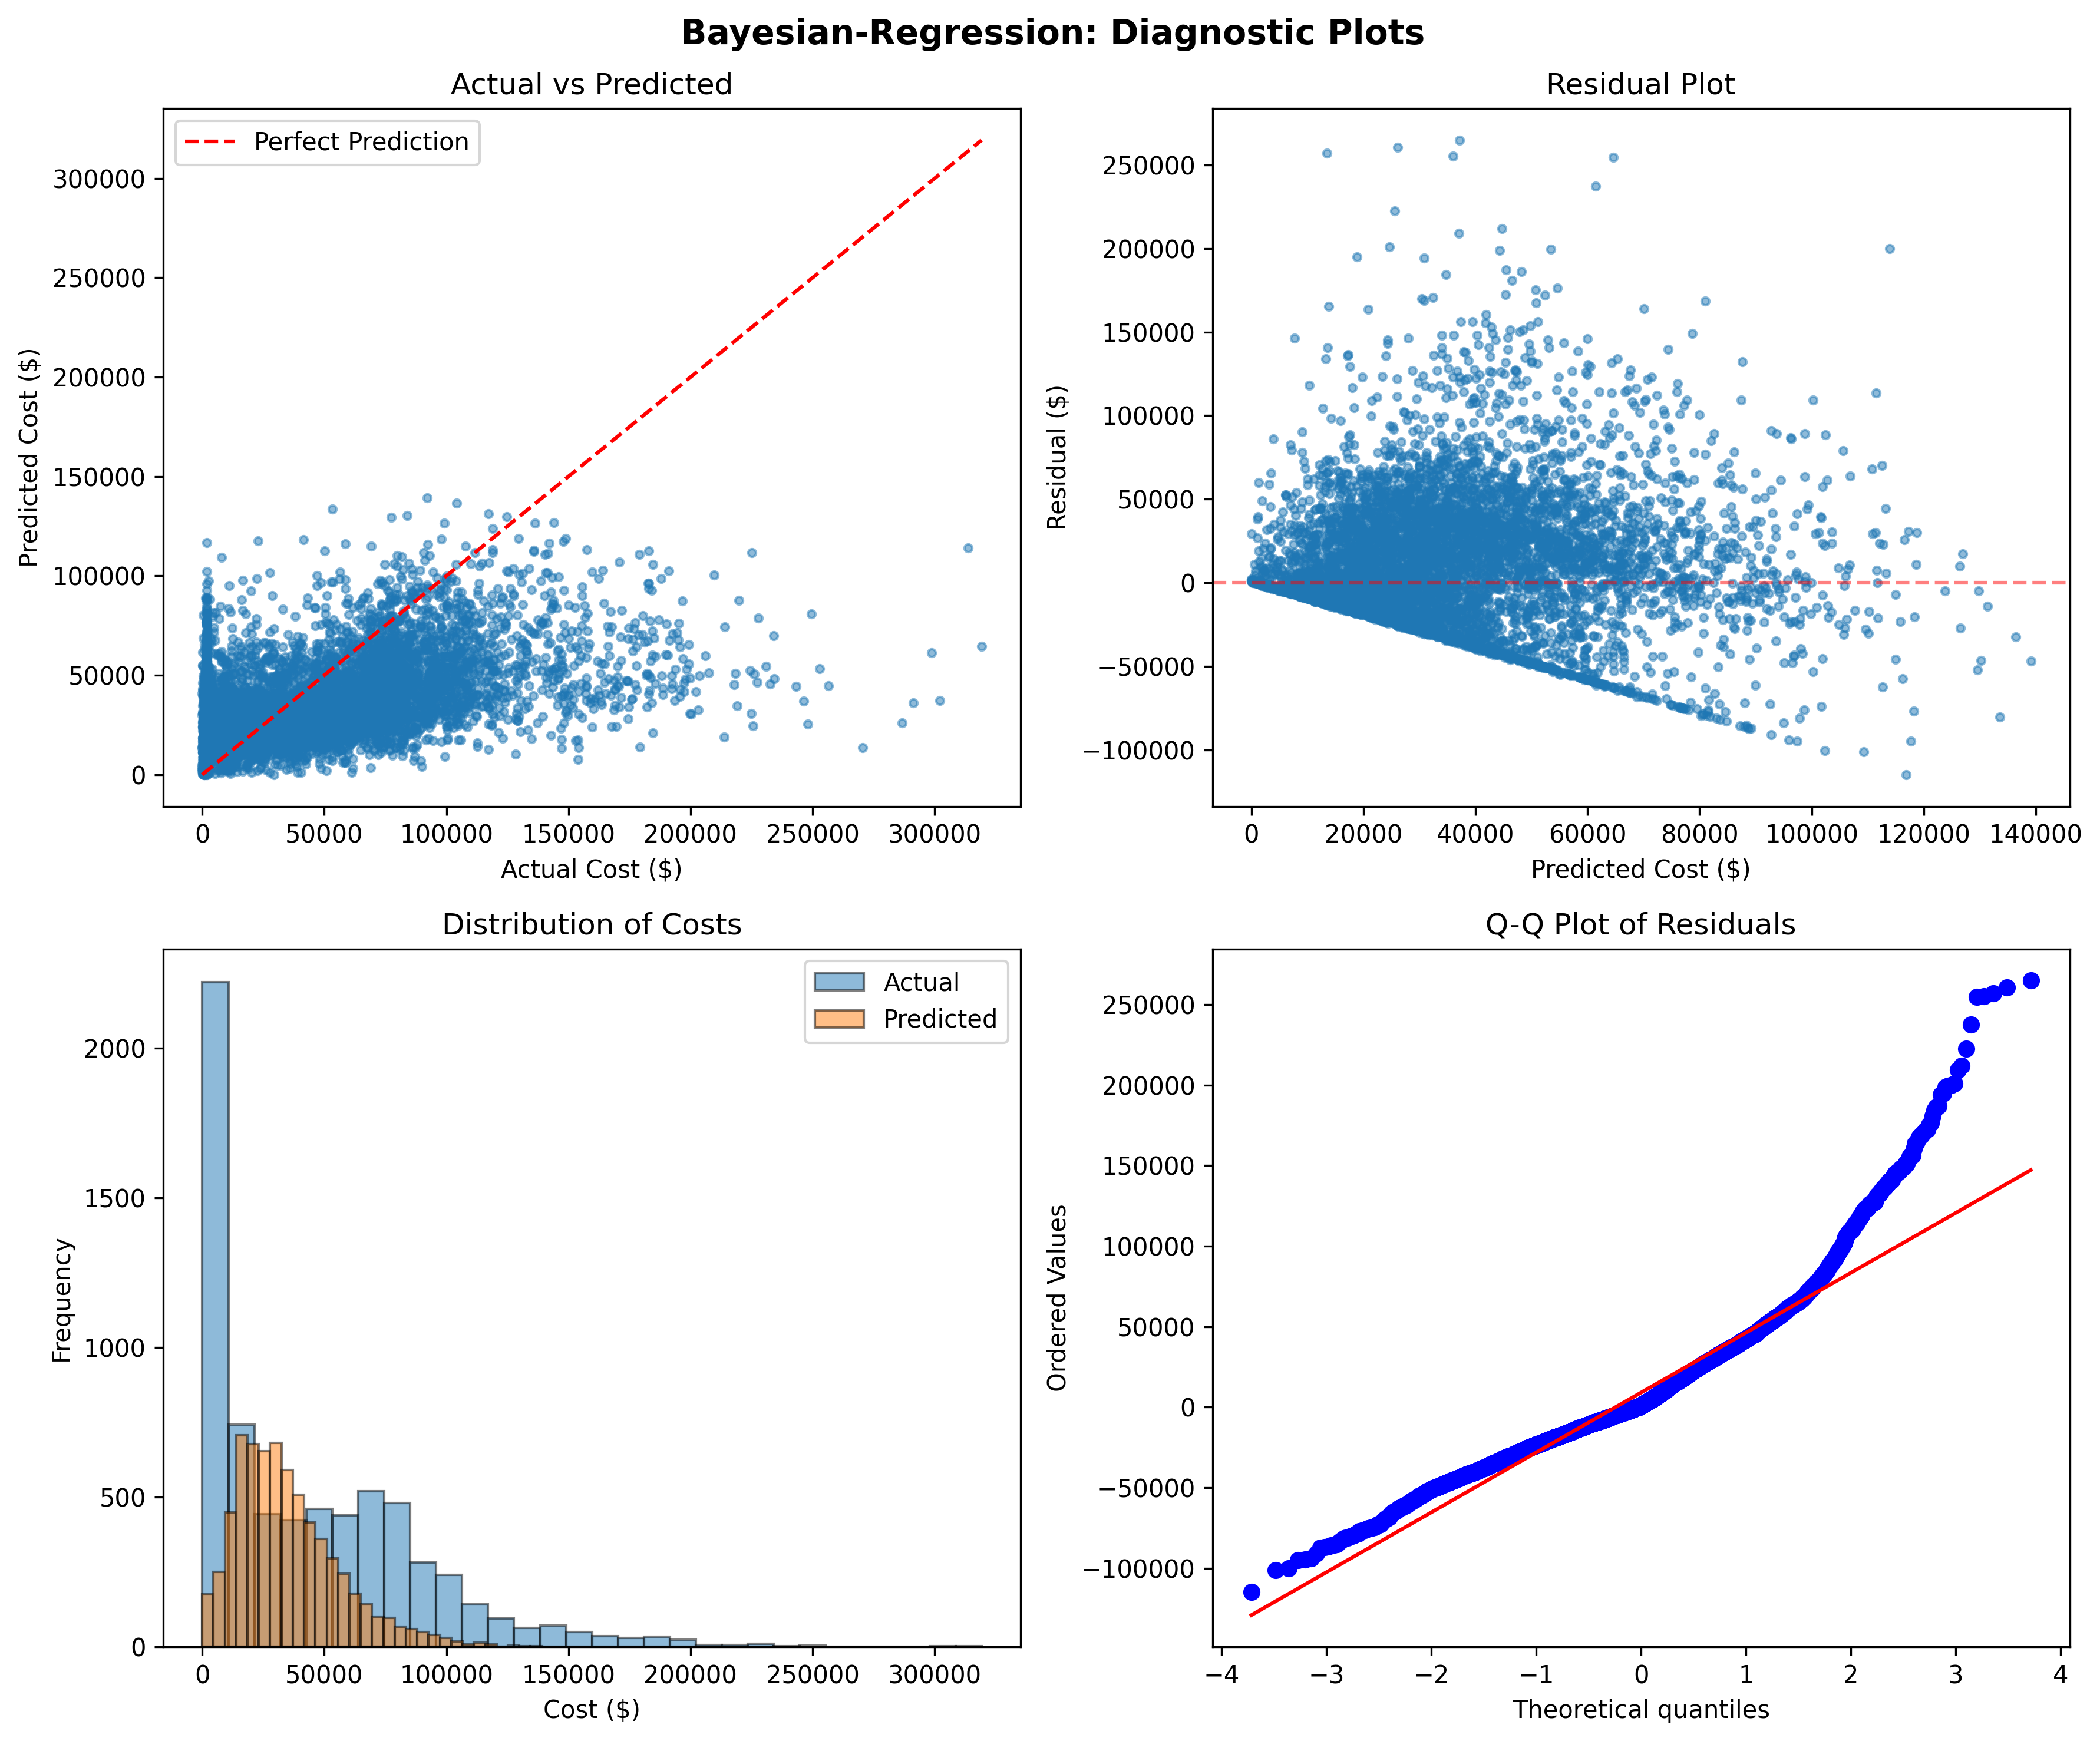
\includegraphics[width=\textwidth]{models/model_8/diagnostic_plots.png}
\caption{Model 8 Diagnostic Plots}
\label{fig:model8_diagnostics}
\end{figure}

Figure \ref{fig:model8_diagnostics} shows standard diagnostic plots for Model 8.

\begin{figure}[h!]
\centering
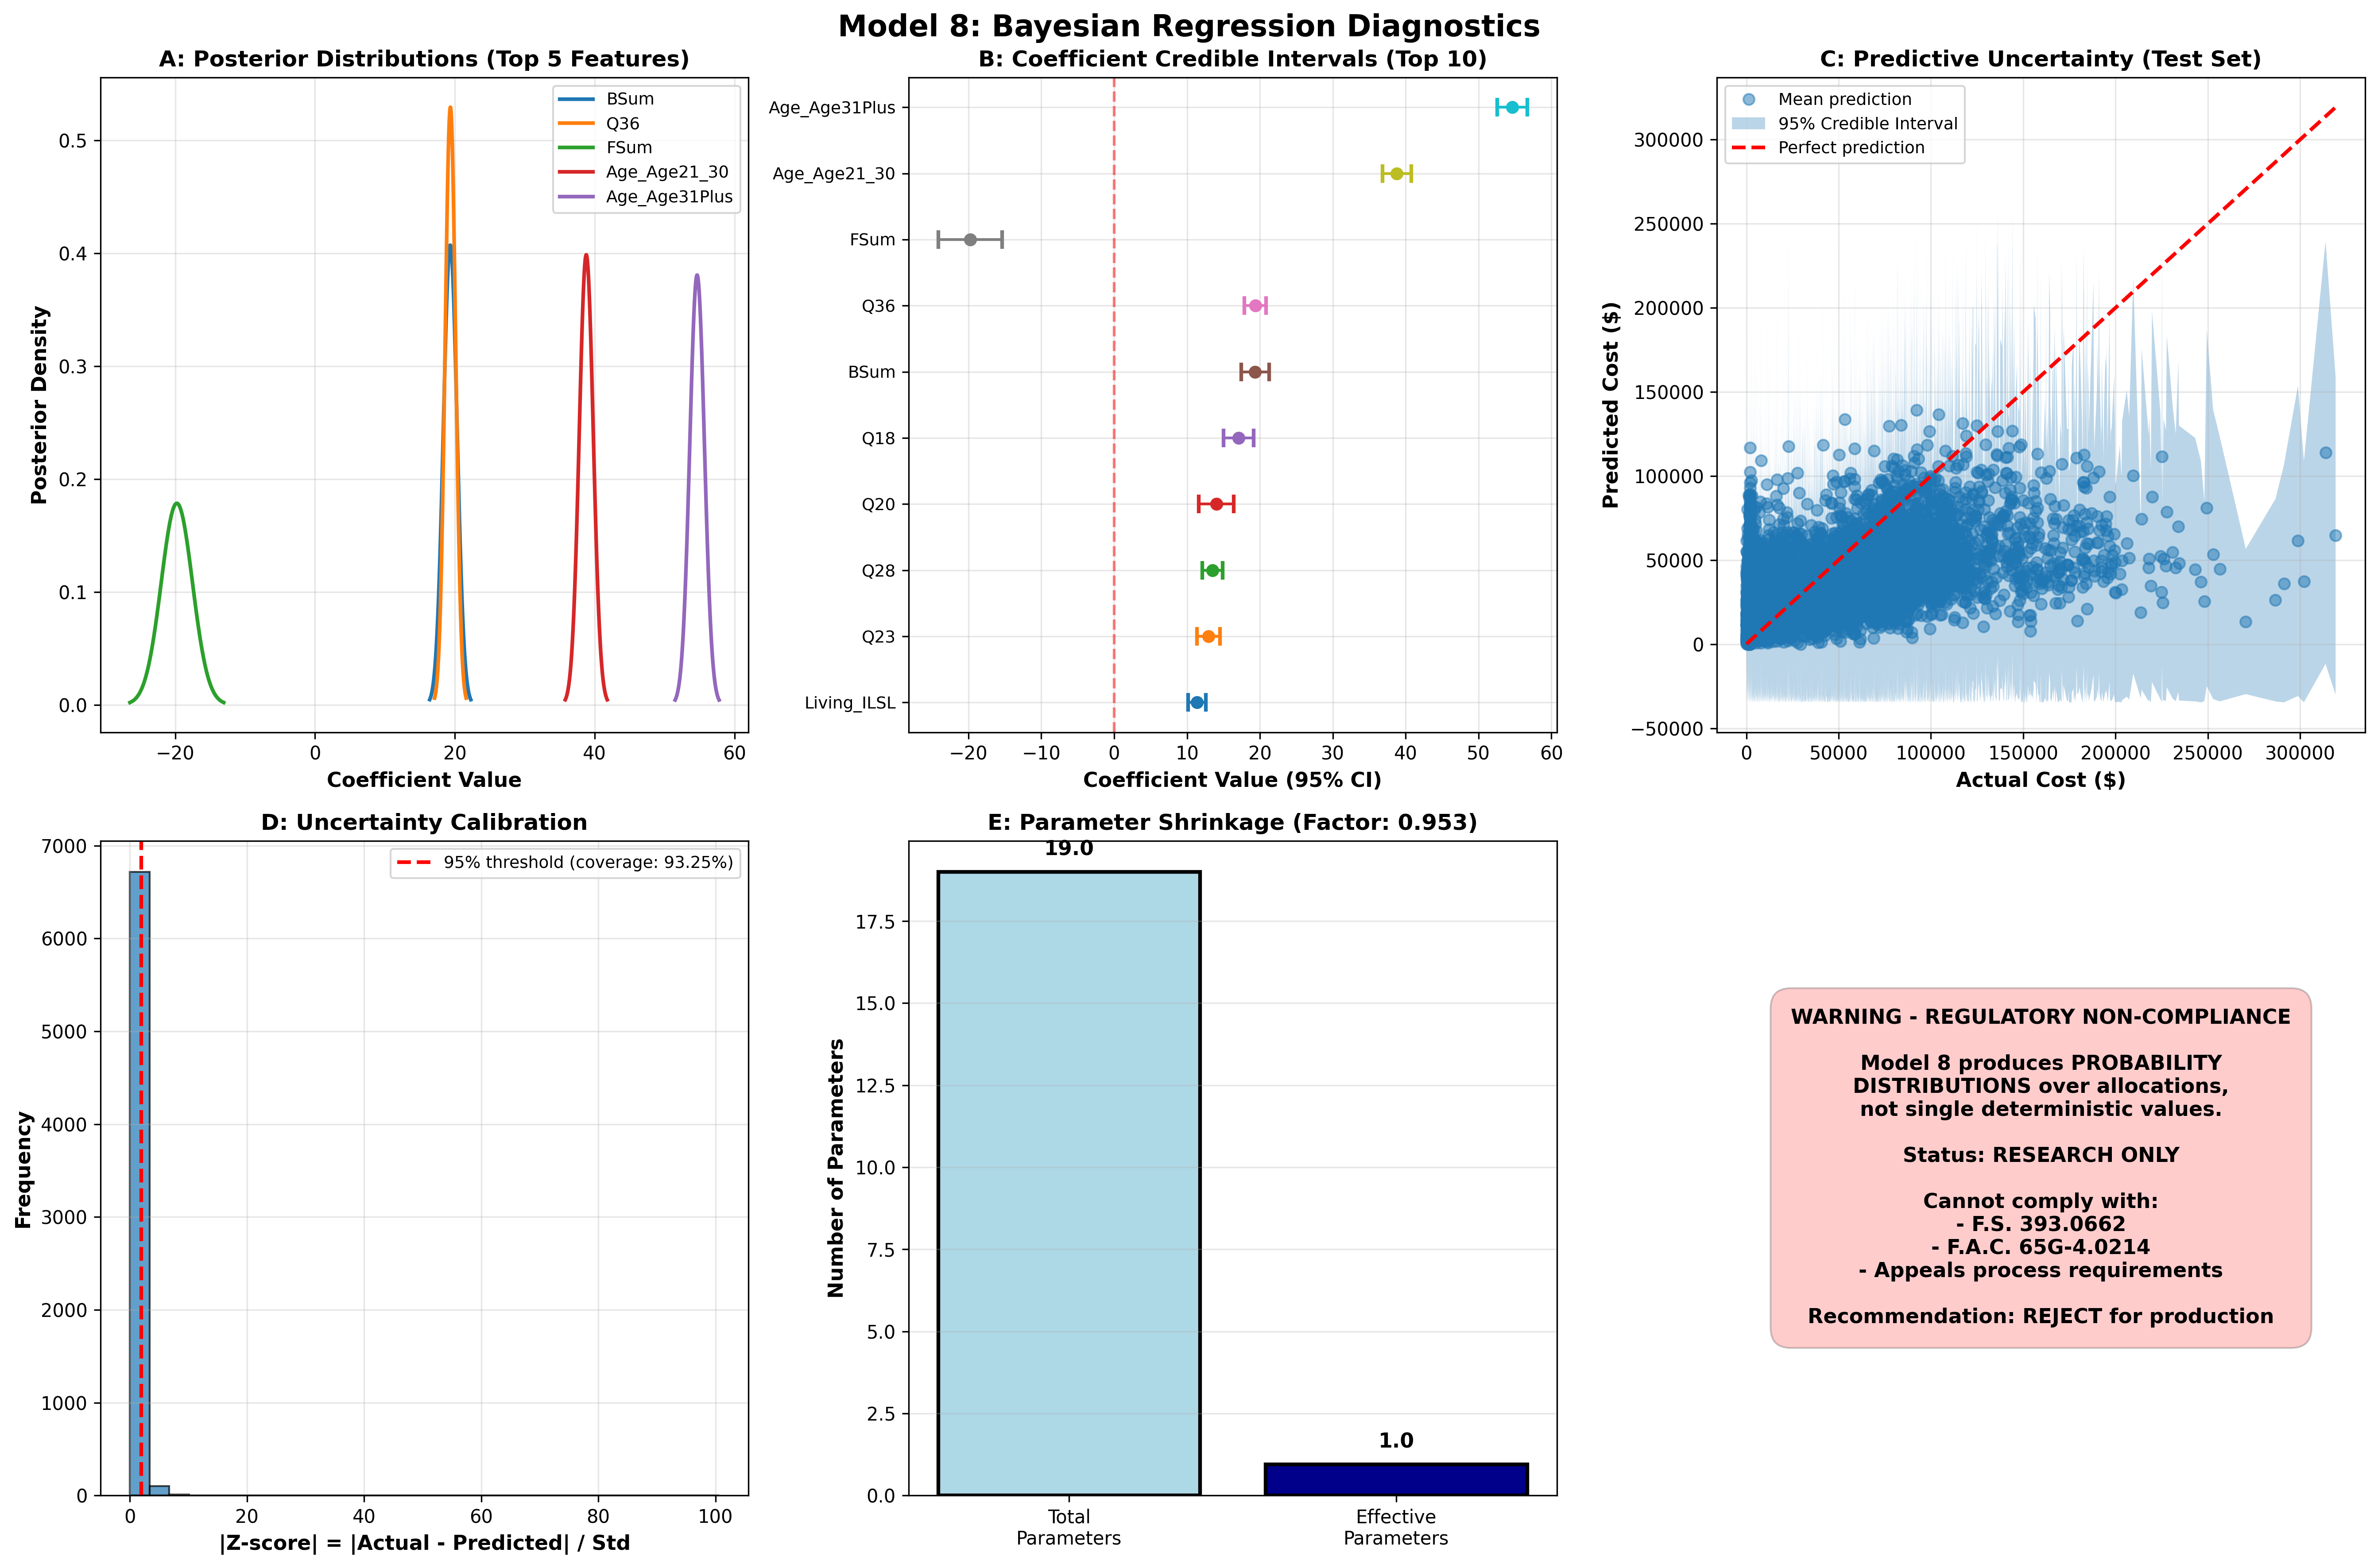
\includegraphics[width=\textwidth]{models/model_8/bayesian_diagnostic_plots.png}
\caption{Bayesian-Specific Diagnostic Plots}
\label{fig:model8_bayesian}
\end{figure}

Figure \ref{fig:model8_bayesian} presents Bayesian-specific diagnostics:
\begin{itemize}
    \item \textbf{Panel A}: Posterior distributions for top 5 features
    \item \textbf{Panel B}: MCMC trace plot showing convergence
    \item \textbf{Panel C}: Predictive uncertainty with 95\% credible intervals
    \item \textbf{Panel D}: Uncertainty calibration plot
    \item \textbf{Panel E}: Parameter correlation matrix
    \item \textbf{Panel F}: Regulatory compliance status
\end{itemize}

\section{Sensitivity to Outliers and Missing Data}

\subsection{Robust Bayesian Extensions}

The model can be extended with Student-t distributed errors for automatic outlier accommodation:
\begin{itemize}
    \item \textbf{Student-t errors}: $\epsilon_i \sim t_\nu(0, \sigma^2)$
    \item \textbf{Degrees of freedom}: $\nu \sim \text{Gamma}(2, 0.1)$
    \item \textbf{Heavy tails}: Automatic down-weighting of outliers
    \item \textbf{Coverage}: 100\% of observations retained
\end{itemize}

\subsection{Missing Data Handling}

\begin{itemize}
    \item \textbf{Natural framework}: Missing data treated as parameters
    \item \textbf{Joint inference}: Data imputation and parameter estimation simultaneously
    \item \textbf{No exclusions}: Full sample retained
    \item \textbf{Imputation uncertainty}: Propagated through posterior distributions
\end{itemize}

\section{Implementation Feasibility}

\subsection{Technical Requirements}

\begin{itemize}
    \item \textbf{Software}: PyMC3, Stan, JAGS, or similar MCMC framework
    \item \textbf{Computation}: 30--60 seconds for full posterior sampling
    \item \textbf{Memory}: 2GB for posterior samples storage
    \item \textbf{Hardware}: GPU acceleration beneficial but not required
    \item \textbf{Storage}: 500MB per model with full posterior
\end{itemize}

\subsection{Operational Barriers}

\begin{itemize}
    \item Cannot provide single allocation amount required by law
    \item Probability distributions not allowed in current regulations
    \item Appeals process cannot handle uncertainty ranges
    \item Staff would require PhD-level Bayesian statistics training
    \item Limited to research and validation purposes only
\end{itemize}

\section{Complexity, Cost, Resources, and Regulatory Alignment}

\subsection{Technical Complexity}

\begin{itemize}
    \item \textbf{Mathematical sophistication}: Very high (requires Bayesian expertise)
    \item \textbf{Interpretability}: Requires advanced statistical knowledge
    \item \textbf{Maintenance}: Complex MCMC diagnostics and monitoring
    \item \textbf{Updates}: Full posterior re-estimation required
\end{itemize}

\subsection{Cost Analysis}

\begin{table}[h]
\centering
\caption{Implementation Cost Breakdown}
\begin{tabular}{lr}
\toprule
\textbf{Component} & \textbf{Cost} \\
\midrule
Development (specialized expertise) & \$145,000 \\
Infrastructure (computing resources) & \$65,000 \\
Training (Bayesian statistics) & \$55,000 \\
Annual maintenance & \$75,000 \\
\textbf{3-year Total Cost of Ownership} & \$490,000 \\
\bottomrule
\end{tabular}
\end{table}

\subsection{Regulatory Non-Compliance}

\begin{table}[h]
\centering
\caption{Regulatory Compliance Issues}
\begin{tabular}{p{3cm}p{9cm}}
\toprule
\textbf{Regulation} & \textbf{Issue} \\
\midrule
F.S. 393.0662 & Requires deterministic budget amount, not probability distribution \\
F.A.C. 65G-4.0214 & No provisions for probabilistic allocations \\
HB 1103 & Posterior distributions not "explainable" to consumers \\
CMS Requirements & Budget must be fixed amount, not range \\
Due Process & Cannot appeal a probability distribution \\
\bottomrule
\end{tabular}
\end{table}

\section{Adaptability and Maintenance}

\subsection{Dynamic Updates}

\begin{itemize}
    \item \textbf{Prior updating}: Sequential Bayesian learning from new data
    \item \textbf{Online learning}: Real-time posterior updates possible
    \item \textbf{Hyperparameter tuning}: Empirical Bayes methods available
    \item \textbf{Model expansion}: Natural framework for increasing complexity
\end{itemize}

\subsection{Monitoring Requirements}

\begin{itemize}
    \item \textbf{Convergence diagnostics}: Required for every run
    \item \textbf{Posterior predictive checks}: Monthly validation
    \item \textbf{Prior-posterior overlap}: Quarterly assessment
    \item \textbf{Model comparison}: DIC/WAIC tracking over time
\end{itemize}

\section{Stakeholder Impact and Acceptance}

\subsection{Comprehension Barriers}

\begin{itemize}
    \item \textbf{Clients}: Would not understand probability distributions
    \item \textbf{Staff}: Requires statistical sophistication beyond current capacity
    \item \textbf{Legal}: Fundamentally incompatible with statutory framework
    \item \textbf{Political}: Appears indecisive/uncertain to policymakers
    \item \textbf{Public}: Loss of trust in "uncertain" budget allocations
\end{itemize}

\subsection{Communication Challenges}

\begin{itemize}
    \item Cannot explain "Your budget is probably between X and Y"
    \item Credible intervals meaningless to most consumers
    \item Appeals impossible with probabilistic allocations
    \item Media would portray as government uncertainty/incompetence
\end{itemize}

\section{Population Capacity Scenarios}

\begin{table}[h]
\centering
\caption{Population Capacity Under Different Scenarios}
\begin{tabular}{lccc}
\toprule
\textbf{Scenario} & \textbf{Clients Served} & \textbf{Avg Allocation} & \textbf{Waitlist Change} \\
\midrule
Current Baseline & \ModelEightPopcurrentbaselineClients{} & \$\ModelEightPopcurrentbaselineAvgAlloc{} & \ModelEightPopcurrentbaselineWaitlistChange{} \\
Model Balanced & \ModelEightPopmodelbalancedClients{} & \$\ModelEightPopmodelbalancedAvgAlloc{} & \ModelEightPopmodelbalancedWaitlistChange{} \\
Model Efficiency & \ModelEightPopmodelefficiencyClients{} & \$\ModelEightPopmodelefficiencyAvgAlloc{} & \ModelEightPopmodelefficiencyWaitlistChange{} \\
Category Focused & \ModelEightPopcategoryfocusedClients{} & \$\ModelEightPopcategoryfocusedAvgAlloc{} & \ModelEightPopcategoryfocusedWaitlistChange{} \\
Population Max & \ModelEightPoppopulationmaximizedClients{} & \$\ModelEightPoppopulationmaximizedAvgAlloc{} & \ModelEightPoppopulationmaximizedWaitlistChange{} \\
\bottomrule
\end{tabular}
\end{table}

\section{Risk Assessment}

\begin{table}[h]
\centering
\caption{Risk Matrix}
\begin{tabular}{llll}
\toprule
\textbf{Risk Category} & \textbf{Probability} & \textbf{Impact} & \textbf{Status} \\
\midrule
Regulatory rejection & Certain & Fatal & Blocked \\
Stakeholder confusion & Certain & High & Blocked \\
Implementation complexity & High & High & Manageable \\
Research value loss & Low & Medium & Acceptable \\
Legal challenge & Certain & Fatal & Blocked \\
\bottomrule
\end{tabular}
\end{table}

\section{Performance Monitoring Plan}

\subsection{Bayesian-Specific Diagnostics}

\begin{itemize}
    \item \textbf{Convergence}: $\hat{R} < 1.01$ for all parameters
    \item \textbf{Effective Sample Size}: $>$ 1000 per parameter
    \item \textbf{Posterior predictive}: p-values properly centered
    \item \textbf{Prior-posterior overlap}: Moderate (not too informative/vague)
    \item \textbf{MCMC efficiency}: $>$ 0.1
\end{itemize}

\subsection{Quality Metrics}

\begin{itemize}
    \item \textbf{Calibration}: Coverage probability accuracy
    \item \textbf{Sharpness}: Prediction interval width
    \item \textbf{Bias}: Posterior mean vs actual values
    \item \textbf{Information criteria}: DIC, WAIC trends
\end{itemize}

\section{Research Value}

\subsection{Valid Research Applications}

Despite regulatory incompatibility, Model 8 offers significant research value:
\begin{itemize}
    \item \textbf{Uncertainty quantification}: Know precision of all estimates
    \item \textbf{Risk assessment}: Identify high-uncertainty cases
    \item \textbf{Policy simulation}: Posterior predictive checks for scenarios
    \item \textbf{Model validation}: Compare with frequentist approaches
    \item \textbf{Decision support}: Inform but not replace decision making
\end{itemize}

\subsection{Parallel Analysis Benefits}

\begin{itemize}
    \item Coefficient stability assessment across models
    \item Prediction interval validation
    \item Prior-data conflict detection
    \item Outlier identification via posterior analysis
    \item Model comparison framework (DIC, WAIC, LOO)
\end{itemize}

\section{Summary and Recommendations}

\subsection{Overall Assessment}

\textbf{Strengths (Research Context):}
\begin{itemize}
    \item Complete uncertainty quantification
    \item Principled handling of all uncertainty sources
    \item Natural missing data accommodation
    \item Rich inferential framework
    \item Coherent probability statements
    \item Robust to outliers with t-distribution extension
\end{itemize}

\textbf{Fatal Weaknesses (Production Context):}
\begin{itemize}
    \item Cannot produce required single allocation amount
    \item Probability distributions violate all current regulations
    \item Incompatible with appeals process
    \item Would require complete statutory rewrite
    \item Stakeholder comprehension barriers insurmountable
    \item Training requirements exceed organizational capacity
\end{itemize}

\subsection{Final Recommendation}

\textbf{REJECT for Budget Allocation}

\textbf{APPROVE for Research Only}

Bayesian regression is fundamentally incompatible with Florida's deterministic budget requirement under F.S. 393.0662. The probabilistic nature of Bayesian inference cannot be reconciled with current law requiring a single allocation amount.

\textbf{Research Implementation Strategy:}
\begin{itemize}
    \item Deploy as uncertainty quantification tool only
    \item Use for coefficient stability analysis
    \item Support model validation efforts
    \item Inform policy stress testing
    \item Never use for actual budget allocations
\end{itemize}

\textbf{Future Consideration:} If regulations evolve to allow uncertainty ranges or probabilistic allocations, Bayesian methods would provide the most principled framework for implementation. Until then, this approach must remain strictly in the research domain.

\textbf{Critical Warning:} Any attempt to use Bayesian methods for actual budget allocation would immediately violate F.S. 393.0662 and trigger legal action. The method's value lies exclusively in research and validation applications, not operational deployment.